\documentclass{birkjour}

\usepackage{amsmath}
\usepackage{amssymb}
\usepackage{amsthm}
\usepackage{graphicx}
\usepackage{float}
\usepackage{url}
%\usepackage{hyperref}

\newtheorem{thm}{Theorem}[section]
 \newtheorem{cor}[thm]{Corollary}
 \newtheorem{lem}[thm]{Lemma}
 \newtheorem{prop}[thm]{Proposition}
 \theoremstyle{definition}
 \newtheorem{defn}[thm]{Definition}
 \theoremstyle{remark}
 \newtheorem{rem}[thm]{Remark}
 \newtheorem*{ex}{Example}
 \numberwithin{equation}{section}

\newcommand{\G}{\mathbb{G}}
\newcommand{\V}{\mathbb{V}}
\newcommand{\Vb}{\mathbb{\overline{V}}}
\newcommand{\W}{\mathbb{W}}
\newcommand{\R}{\mathbb{R}}
\newcommand{\B}{\mathbb{B}}

\newcommand{\Alpha}{A}
%\Omega is already defined

\newcommand{\nvao}{o}
\newcommand{\nvai}{\infty}
\newcommand{\nvaob}{\overline{o}}
\newcommand{\nvaib}{\overline{\infty}}

\newcommand{\eminus}{e_{-}}
\newcommand{\eplus}{e_{+}}
\newcommand{\eminusb}{\overline{e}_{-}}
\newcommand{\eplusb}{\overline{e}_{+}}

\newcommand{\Gi}{\dot{G}}
\newcommand{\Go}{\hat{G}}

\begin{document}

\title{A Variation Of The Quadric Model\\Of Geometric Algebra}

\author{Spencer T. Parkin}
\email{spencer.parkin@gmail.com}

\numberwithin{equation}{section}

\subjclass{Primary 14J70; Secondary 14J29}

\keywords{Quadric Surface, Quartic Surface, Geometric Algebra, Quadric Model, Conformal Model}

%\dedicatory{To Melinda and Naomi}

\begin{abstract}
A variation of the quadric model set forth in \cite{Parkin12} is
found in which the rigid body motions are represented by
versors applicable to any quadric surface.
Extending this variation of the original model to include
a specific form of quartic surface, we find that such surfaces are
closed under the application of all conformal transformations.
Results of a computer program implementing this new model are presented.
\end{abstract}

\maketitle

\section{Introduction}

In the original paper \cite{Parkin12}, a model for quadric surfaces was
presented based upon the ideas of projective geometry.  What was unfortunate
about this model, however, was its lack of support for the rigid body transformations.  It was
predicted in the conclusion of that paper that a better model for quadric
surfaces may exist that is more like the conformal model of geometric algebra, here-after
abbreviated CGA.
The present paper details what may be such a model.  We'll find that the rigid
body transformations can be incorporated into the model by using an alternative
method of encoding the quadric form.  An extension to this quadric form
will then allow us to support the conformal transformations at the expense of
expanding our model to necessarily include a specific form of quartic surfaces.  The
new model and its extension will both use the same geometric algebra to be given as follows.

\section{The Geometric Algebra}

We begin here with a description of the structure of the geometric algebra upon
which our model will be imposed.  This
geometric algebra will contain the following vector spaces.
\begin{equation}\label{equ_vector_spaces}
\begin{array}{ll}
\mbox{Notation} & \mbox{Basis} \\
\hline
\V^e & \{e_i\}_{i=1}^n \\
\V^{\nvao} & \{\nvao\}\cup\{e_i\}_{i=1}^n \\
\V^{\nvai} & \{e_i\}_{i=1}^n\cup\{\nvai\} \\
\V & \{\nvao\}\cup\{e_i\}_{i=1}^n\cup\{\nvai\}
\end{array}
\end{equation}
The set of vectors $\{e_i\}_{i=1}^n$ forms an orthonormal set of basis
vectors for the $n$-dimensional Euclidean vector space $\V^e$, which we'll
use to represent $n$-dimensional Euclidean space.
The vectors $\nvao$ and $\nvai$ are the familiar null-vectors representing the
points at origin and infinity, respectively, taken from CGA.
An inner-product table for these basis vectors is given as follows, where
$1\leq i<j\leq n$.
\begin{equation}
\begin{array}{c|cccc}
\cdot & \nvao & e_i & e_j & \nvai \\
\hline
\nvao & 0 & 0 & 0 & -1 \\
e_i & 0 & 1 & 0 & 0 \\
e_j & 0 & 0 & 1 & 0 \\
\nvai & -1 & 0 & 0 & 0
\end{array}
\end{equation}
We will now let $\G(\V)$ denote the Minkowski geometric algebra generated by $\V$.
For each vector space in table \eqref{equ_vector_spaces}, we will let an over-bar
above this vector space denote an identical copy of that vector space.  The vector
space $\W$ will denote the smallest vector space containing each of $\V$ and $\Vb$
as vector subspaces.  In symbols, one may write
\begin{equation}
\G(\W) = \G(\V\oplus\Vb).
\end{equation}

We will use over-bar notation to distinguish between vectors taken from $\V$
with vectors taken from $\Vb$.  For algebraic purposes, we will find it useful
to see that the over-bar notation may be defined as an outermorphic function
that is also an isomorphism between $\G(\V)$ and $\G(\Vb)$.
Doing so, we see that for any element $E\in\G(\V)$,
we may define $\overline{E}\in\G(\Vb)$ as
\begin{equation}\label{equ_over_bar_func}
\overline{E} = SES^{-1},
\end{equation}
where $S\in\G(\W)$ is the element\footnote{The equivalent of $S$ given in \cite{Parkin12}
was erroneously referred to as a versor.} given by
\begin{equation}\label{equ_isomorphism_versor}
S = (1+\eminus\eminusb)(1-\eplus\eplusb)\prod_{i=1}^n(1-e_i\overline{e}_i).
\end{equation}
This definition is non-circular if we let the over-bars in equation \eqref{equ_isomorphism_versor}
be purely notation.  The vectors $\eminus$ and $\eplus$, taken from \cite{LiRockwood},
are defined as
\begin{align}
\eminus &= \frac{1}{2}\nvai + \nvao, \\
\eplus &= \frac{1}{2}\nvai - \nvao.
\end{align}
The vectors $\eminusb$ and $\eplusb$ are defined similarly in terms of $\nvaob$ and $\nvaib$.
Defined this way, realize that, like the over-bar function defined in \cite{Parkin12},
here we have the property that for any vector $v\in\V$, we have $\overline{\overline{v}}=-v$.
Letting $E$ be any element in $\G(\W)$ in equation \eqref{equ_over_bar_func},
we extend the over-bar function to be defined on all of $\G(\W)$.

\section{The Form Of Quadric Surfaces In $\G(\W)$}

We now give a formal definition under which elements $E\in\G(\W)$
are representative of $n$-dimensional quadric surfaces in our present variation
of the original model.
\begin{defn}\label{def_quadric}
Referring to an element $E\in\G(\W)$ as a quadric surface, it is representative of such an $n$-dimensional surface as\footnote{Throughout this paper, we let the outer product take precedence
over the inner product, and the geometric product take precedence over the inner and
outer products.  The inner product used is that given in \cite{Dorst07}, appendix B,
equation (B.1).} the set of all points $p\in\V^o$ such that
\begin{equation}\label{equ_quadric_equation}
0 = p\wedge\overline{p}\cdot E.
\end{equation}
\end{defn}
From this definition it can be seen that the general form of a quadric $E\in\G(\W)$ is given by
\begin{equation}\label{equ_quadric_form}
E = \sum_{i=1}^k a_i\overline{b}_i,
\end{equation}
where each of $\{a_i\}_{i=1}^k$ and $\{b_i\}_{i=1}^k$ is a sequence of $k$ vectors
taken from $\V^\nvai$.  To see why, realize that the form \eqref{equ_quadric_form} can
always be reduced to the form
\begin{equation}\label{equ_quadric_reduced_form}
E \equiv \sum_{i=1}^n\sum_{j=i}^n\lambda_{ij}e_i\overline{e}_j+
\sum_{i=1}^n\lambda_i e_i\nvaib+
\lambda\nvai\nvaib,
\end{equation}
where each of $\lambda_{ij}$, $\lambda_i$, and $\lambda$ are scalars, in the
sense that this reduced form represents the same surface as that in equation \eqref{equ_quadric_form}
under Definition~\ref{def_quadric}.
We then see that this form \eqref{equ_quadric_reduced_form}, when it is
substituted into equation \eqref{equ_quadric_equation}, reduces to a polynomial
equation of degree 2 in the vector components of $p+(p\cdot\nvai)\nvao$.
Doing so with $p=\nvao+x$, where $x\in\V^e$, we get the equation
\begin{equation}\label{equ_quadric_polynomial_equation}
0 = -\sum_{i=1}^n\sum_{j=i}^n\lambda_{ij}(x\cdot e_i)(x\cdot e_j)
+\sum_{i=1}^n\lambda_i(x\cdot e_i) - \lambda,
\end{equation}
which we may recognize as the general equation of an $n$-dimensional quadric surface.
It may be worth comparing this method of representing quadric surfaces with that done
in chapter 4 of \cite{Li08} in what is called a quadratic Grassmann-Caylay algebra.

In practice, a computer program might take such a bivector of the form \eqref{equ_quadric_form}
and extract from it the coefficients of the quadric
polynomial \eqref{equ_quadric_polynomial_equation} it
represents.  It could then render the surface using traditional methods, such as those used
to render the traced surfaces in Figure~\ref{fig_invert_cylinder_in_sphere_wire} far below,
or the meshed surfaces in Figure~\ref{fig_invert_cylinder_in_sphere_solid} yet further below.

Of course, using geometric algebra on paper, it might be undesirable and unnecessary to think of
quadrics in terms of polynomial equations.  A, perhaps, better way to think of quadrics is in terms
of an element of a geometric algebra whose decomposition
produces the parameters characterizing the quadric surface.  For example, many common
quadrics, such as the cylinder, double-cone, spheroid and hyperboloid of two sheets, are the
solution set in $\V^e$ of the equation
\begin{equation}
0 = -r^2 + (x-c)^2 + \lambda((x-c)\cdot v)^2
\end{equation}
in the variable $x$.  (An explanation of the parameters $r$, $c$, $v$ and $\lambda$
was given in \cite{Parkin12}.)  Then, factoring out $-p\overline{p}$, we see that
the element $E\in\G(\W)$, given by
\begin{equation}\label{equ_canonical_form_of_common_quadric}
E=\Omega + \lambda v\overline{v}+2(c+\lambda(c\cdot v)v)\nvaib+
(c^2+\lambda (c\cdot v)^2-r^2)\nvai\nvaib
\end{equation}
is representative of this very same quadric by Definition~\ref{def_quadric},
where $\Omega$ is defined as
\begin{equation}
\Omega = \sum_{i=1}^n e_i\overline{e}_i.
\end{equation}
Canonical forms similar to \eqref{equ_canonical_form_of_common_quadric}
can be found for specific geometries, such as planes, spheres, plane-pairs,
circular cylinders, circular conical surfaces, and so on.

\section{Transformations Supported By The Model}

The main result of this section will depend upon the following lemma.
\begin{lem}\label{lma_versor_transfer}
For any versor $V\in\G(\W)$, and any four vectors $a,b,c,d\in\V$, we have
\begin{equation}
V^{-1}aV\wedge\overline{V^{-1}bV}\cdot c\wedge\overline{d} =
a\wedge\overline{b}\cdot V\overline{V}(c\wedge\overline{d})(V\overline{V})^{-1}.
\end{equation}
\end{lem}
\begin{proof}
We begin by first establishing that
\begin{align}
 & V^{-1}aV\wedge\overline{V^{-1}bV}\cdot c\wedge\overline{d} \\
=\;& -(V^{-1}aV\cdot c)(V^{-1}bV\cdot d) \\
=\;& -(a\cdot VcV^{-1})(b\cdot VdV^{-1}) \\
=\;& a\wedge\overline{b}\cdot VcV^{-1}\wedge\overline{VdV^{-1}}.
\end{align}
We now notice that
\begin{align}
& VcV^{-1} \\
=\;& V\overline{VV^{-1}}cV^{-1} \\
=\;& (-1)^m V\overline{V}c\overline{V^{-1}}V^{-1} \\
=\;& (-1)^m V\overline{V}c(V\overline{V})^{-1},
\end{align}
where $m$ is the number of vectors taken together in a geometric
product to form $V$.  We then notice that
\begin{align}
& \overline{VdV^{-1}} \\
=\;& VV^{-1}\overline{VdV^{-1}} \\
=\;& (-1)^{m^2}V\overline{V}V^{-1}\overline{dV^{-1}} \\
=\;&(-1)^{m^2+m}V\overline{Vd}V^{-1}\overline{V^{-1}} \\
=\;&(-1)^{2m^2+m}V\overline{VdV^{-1}}V^{-1} \\
=\;&(-1)^mV\overline{Vd}(V\overline{V})^{-1}.
\end{align}
It now follows that
\begin{align}
 & a\wedge\overline{b}\cdot VcV^{-1}\wedge\overline{VdV^{-1}} \\
=\;& a\wedge\overline{b}\cdot (-1)^{2m}V\overline{V}c(V\overline{V})^{-1}\wedge V\overline{Vd}(V\overline{V})^{-1} \\
=\;& a\wedge\overline{b}\cdot V\overline{V}(c\wedge\overline{d})(V\overline{V})^{-1},
\end{align}
which completes the proof.
\end{proof}
We're now ready to prove the main result as follows.
\begin{lem}\label{lma_quadric_transform}
Letting $E\in\G(\W)$ be a bivector of the form \eqref{equ_quadric_form},
$p,p'\in\V^o$ be a pair of points related by a versor $V\in\G(\V)$ by
the equation
\begin{equation}\label{equ_get_rid_ni}
p' = \nvao\cdot V^{-1}pV\wedge\nvai,
\end{equation}
and $E'\in\G(\W)$ a bivector given by
\begin{equation}\label{equ_transformed_surface}
E' = V\overline{V}E(V\overline{V})^{-1},
\end{equation}
the set of all points $p\in\V^\nvao$ such that
\begin{equation}\label{equ_wanted_set}
0 = p'\wedge\overline{p}'\cdot E
\end{equation}
is exactly the set of all points $p\in\V^\nvao$ such that
\begin{equation}\label{equ_derived_set}
0 = p\wedge\overline{p}\cdot E'.
\end{equation}
\end{lem}
\begin{proof}
The lemma goes through by the following chain of equalities.
\begin{align}
 & (\nvao\cdot V^{-1}pV\wedge\nvai)\wedge\overline{(\nvao\cdot V^{-1}pV\wedge\nvai)}\cdot E \\
=\;& V^{-1}pV\wedge\overline{V^{-1}pV}\cdot E \\
=\;& p\wedge\overline{p}\cdot(V\overline{V})E(V\overline{V})^{-1}.
\end{align}
The first equality holds by the fact that $E$ is of the form \eqref{equ_quadric_form},
while the second equality holds by Lemma~\ref{lma_versor_transfer}.
\end{proof}
A corrollary to Lemma~\ref{lma_quadric_transform} immediately follows.
\begin{cor}\label{cor_quadric_transform}
If $V\in\G(\V)$ is a versor such that $E'$ in equation \eqref{equ_transformed_surface}
is of the form \eqref{equ_quadric_form}, then the versor $V\overline{V}$
represents a transformation closed in the set of all quadric surfaces.
\end{cor}

The key motivation behind Lemma~\ref{lma_quadric_transform} is
the observation that the desired transformation of $E$ by $V$ is
given by the algebraic set of equation \eqref{equ_wanted_set}, because
an understanding of how $V^{-1}$ transforms $p$ gives us an understanding
of what type of geometry we get from equation \eqref{equ_wanted_set} in terms of
$E$ and $V$.  Lemma~\ref{lma_quadric_transform} then
shows that this is also the algebraic set of equation \eqref{equ_derived_set}, thereby
giving us a means of performing desired transformations on elements in $\G(\W)$ representative
of quadric surfaces.
By Corrollary~\ref{cor_quadric_transform}, what we get
from such a transformation is also a quadric surface, provided that $V$ is a
versor such that $E'$
in \eqref{equ_transformed_surface}, like $E$, is also a bivector of the form \eqref{equ_quadric_form}.

We can now apply Lemma~\ref{lma_quadric_transform} to show
that the rigid body transformations are supported in our new variation
of the original model.
Letting $\pi\in\V$ be a dual plane of CGA, given by
\begin{equation}
\pi = v+(c\cdot v)\nvai,
\end{equation}
where $v\in\V^e$ is a unit-length vector indicating the norm of the plane,
and where $c\in\V^e$ is a vector representing a point on the plane,
we see that for any homogenized point $p\in\V^o$, we have
\begin{equation}
-\pi p\pi^{-1} = \nvao+x-2((x-c)\cdot v)v + \lambda\nvai,
\end{equation}
where $p=\nvao+x$ with $x\in\V^e$, and
where the scalar $\lambda\in\R$ is of no consequence.  Letting $V=\pi$,
the point $p'\in\V^o$ of consequence here is given by equation \eqref{equ_get_rid_ni},
from which we can recognize an orthogonal reflection about the plane $\pi$.
It now follows by Lemma~\ref{lma_quadric_transform} that $\pi\overline{\pi}$ is a versor
capable of reflecting any quadric surface about the plane $\pi$.
Being able to perform planar reflections of any quadric in any plane, it
now follows that we can always find a versor $V\in\G(\W)$ capable of performing
any rigid body motion on any quadric surface.  The development
of the rigid body motions, (combinations of translations and rotations), by planar reflections,
is well known, and can be found in section 2.7 of \cite{LiRockwood}.

In retrospect, what we have done to find the rigid body motions
of quadric surfaces is similar to what was done in \cite{Langer08}; and
according to \cite{Pfister95}, we can state more generally that what we
have done is at least similar to finding an isomorphism between quadratic spaces.
Section 4 of \cite{Lasenby05} shows that versors can be used to transform quadric
surfaces using an entirely different approach.

\section{Extending The New Model}

\begin{figure}
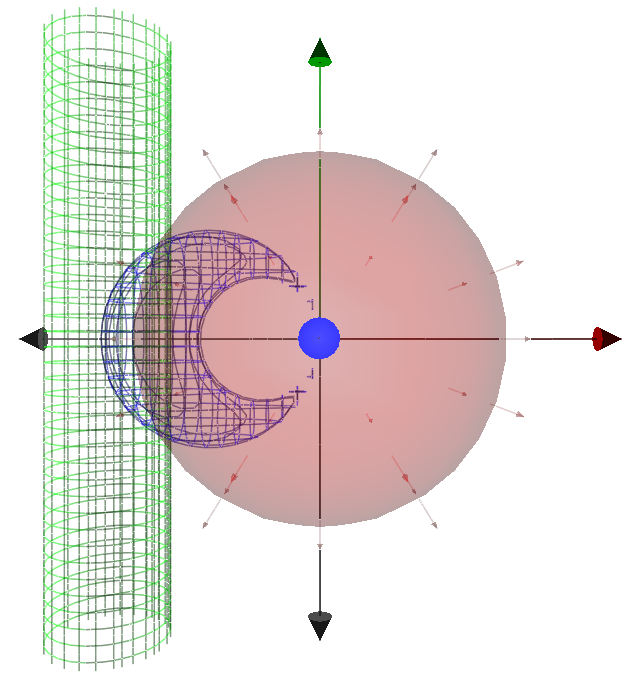
\includegraphics[scale=0.3]{InvertCylinderInSphereWire}
\caption{The inversion of a cylinder in a sphere.  Traces in various planes were
used to render the cylinder and its inversion.}
\label{fig_invert_cylinder_in_sphere_wire}
\end{figure}
\begin{figure}
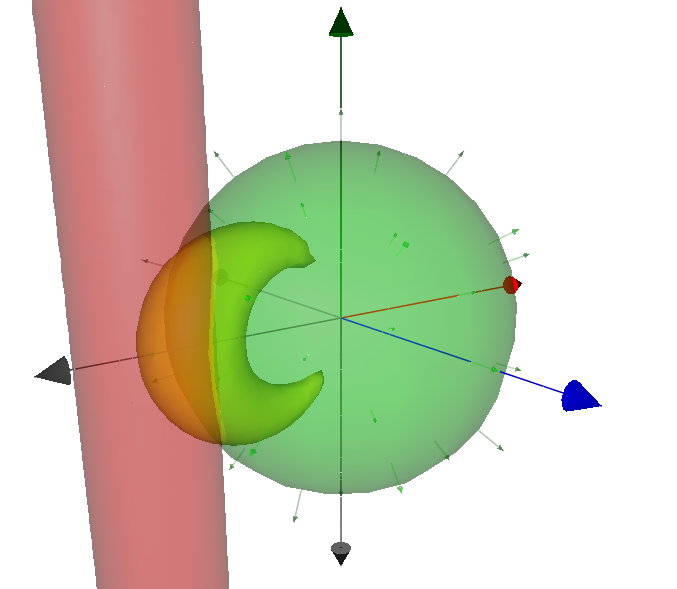
\includegraphics[scale=0.3]{InvertCylinderInSphereSolid}
\caption{The inversion of a cylinder in a sphere.  A surface mesh generation
algorithm was used to skin the cylindrical and inverted surfaces.  The inverted
mesh suffers where the curvature becomes extreme.}
\label{fig_invert_cylinder_in_sphere_solid}
\end{figure}
Interestingly, if we were not content with the rigid body motions of
quadrics, then we really could find what is, for example, the spherical
inversion of, say, an infinitely long cylinder in a sphere.  To do this, we start by changing
Definition~\ref{def_quadric} into the following definition.
\begin{defn}\label{def_surface}
For any element $E\in\G(\W)$, we may refer to it as an $n$-dimensional
quartic surface as the set of all points $p\in\V^e$ such that
\begin{equation}\label{equ_surface_set}
0 = P(p)\wedge\overline{P}(p)\cdot E,
\end{equation}
where $P:\V^e\to\V$ is the point mapping of CGA, defined in \cite{Hestenes01} as
\begin{equation}\label{equ_cga_point_map}
P(p) = \nvao + p + \frac{1}{2}p^2\nvai.
\end{equation}
\end{defn}
It is then helpful to introduce another definition as follows.
\begin{defn}\label{def_preserve_point_map}
A versor $V\in\G(\V)$ is said to be point-form preserving if for
any point $x\in\V^e$, there exists a non-zero scalar $\lambda\in\R$ and
a point $y\in\V^e$ such that $V^{-1}P(x)V=\lambda P(y)$.
\end{defn}
We then arrive at the following upgrade of Lemma~\ref{lma_quadric_transform}.
\begin{lem}\label{lma_quartic_transform}
Letting $E\in\G(\W)$ be a bivector of any form, $p,p'\in\V^e$ be
a pair of points related by a point-form preserving versor $V\in\G(\V)$ by
the equation
\begin{equation}
\lambda P(p') = V^{-1}P(p)V,
\end{equation}
and $E'\in\G(\W)$ a bivector given by equation \eqref{equ_transformed_surface},
the set of all point $p\in\V^e$ such that
\begin{equation}\label{equ_wanted_set2}
0 = P(p')\wedge\overline{P}(p')\cdot E
\end{equation}
is exactly the set of all point $p\in\V^e$ such that
\begin{equation}
0 = P(p)\wedge\overline{P}(p)\cdot E'.
\end{equation}
\end{lem}
\begin{proof}
The scalar $\lambda$ clearly divides out of equation \eqref{equ_wanted_set2} so that we may,
without loss of generality, let $\lambda=1$.
Once again applying Lemma~\ref{lma_versor_transfer}, we simply see that
\begin{equation}
V^{-1}P(p)V\wedge\overline{V^{-1}P(p)V}\cdot E = P(p)\wedge\overline{P}(p)\cdot V\overline{V}E(V\overline{V})^{-1}.
\end{equation}
\end{proof}

The need for a point-form preserving versor is apparent from equation
\eqref{equ_wanted_set2}, since otherwise we could not claim to understand what
algebraic set we get from equation \eqref{equ_wanted_set2} in terms of $E$ and $V$.
We now see by Lemma~\ref{lma_quartic_transform}
that if $V\in\G(\W)$ is any point-form preserving versor, and if $E$
is a surface under Definition~\ref{def_surface}, then the element $E'\in\G(\W)$,
given by equation \eqref{equ_transformed_surface}, must, by Definition~\ref{def_surface},
be representative of the desired transformation of $E$ by the versor $V\overline{V}$.
The general polynomial equation arising from the form of
such elements $E$ in Defintion~\ref{def_surface} is much more involved than
what we have in equation \eqref{equ_quadric_polynomial_equation}.  Nevertheless, it is possible to extract
a specific form of a quartic polynomial equation in
the vector components of $p$ from equation \eqref{equ_surface_set}.
The result being unsightly, it will not be presented here.  Suffice it to say, a computerized
algebra system was used to find the polynomial form.  In any case, it is easy
to see from equation \eqref{equ_surface_set} that the degree of the resulting
polynomial will be four.

Now notice that under Definition~\ref{def_surface}, canonical forms
such as \eqref{equ_canonical_form_of_common_quadric} are still valid.
This is because
\begin{equation}
P(p)\wedge\overline{P}(p)\cdot E = (\nvao+p)\wedge\overline{(\nvao+p)}\cdot E
\end{equation}
in the case that $E$ is of the form \eqref{equ_quadric_form}.  This allows
us to use what we already know about quadrics in the new model with its extension to
quartic surfaces of a specific form.

An interesting side effect of Definition~\ref{def_surface} is the existence
of every union of any pair of geometries where either one is a circle, plane
or point.  We simply note that for any pair of vectors $a,b\in\V$, we have
\begin{equation}
P(p)\wedge\overline{P}(p)\cdot a\wedge\overline{b} = -(P(p)\cdot a)(P(p)\cdot b).
\end{equation}

Putting theory into practice, the author wrote a piece of computer
software\footnote{The software is available
at \url{https://github.com/spencerparkin/GAVisTool}.  The author does
not recommend making use of this software for research purposes.  Instead,
the reader is referred to tools such as GAViewer and CLUCalc.}
that implements this CGA-like model for the special class of
quartic surfaces of equation \eqref{equ_surface_set}.  Giving the program the following
script as input, the output of the program is given in
Figure~\ref{fig_invert_cylinder_in_sphere_wire} and rendered another way in
Figure~\ref{fig_invert_cylinder_in_sphere_solid}.
The script is easy for anyone to read, even if they are not familiar with its language.  It is given
here to illustrate how one might use the model with the aide a computer system.
%\begin{samepage}
\begin{center}
{\tiny
\begin{verbatim}

/*
 * Calculate the surface that is the
 * inversion of a cylinder in a sphere.
 */
do
(
    /* Make the cylinder. */
    v = e2, c = -7*e1, r = 2,
    cylinder = Omega - v^bar(v) + 2*c*nib + (c.c - r*r)*ni^nib,
    bind_quadric(cylinder),
    geo_color(cylinder,0,1,0),
	
    /* Make the sphere. */
    c = 0, r = 6,
    sphere = no + c + 0.5*(c.c - r*r)*ni,
    bind_dual_sphere(sphere),
    geo_color(sphere,1,0,0,0.2),
	
    /* Make the inversion of the cylinder in the sphere. */
    V = sphere*bar(sphere),
    inversion = V*cylinder*V~,
    bind_conformal_quartic(inversion),
    geo_color(inversion,0,0,1),
)

\end{verbatim}
}
\end{center}
%\end{samepage}
The language used here was invented for the software and has no name.
The functions beginning with the word ``bind'' create and bind an entity to the given
element of the geometric algebra that is responsible for interpreting that element
as a surface under Definition~\ref{def_surface} or, in the case of the sphere, as a dual surface under the definition
given by CGA.  The computer program can then
use traditional methods to render the surface from the extracted polynomial equation.
For example, the polynomial equation in $x$, $y$ and $z$ for the inverted surface presented
in Figure~\ref{fig_invert_cylinder_in_sphere_wire} is given by
\begin{equation}
\begin{split}
0 =\;& 28.8x^{2} + 11.2x^{3} + x^{4} + 11.2xy^{2} + 2x^{2}y^{2} + \\
 & 11.2xz^{2} + 2x^{2}z^{2} + y^{4} + 2y^{2}z^{2} + 28.8z^{2} + z^{4}.
\end{split}
\end{equation}
It is interesting how a bit of reasoning in geometric algebra has given us such a simple means
to obtaining this polynomial equation.
Of course, while such equations lend themselves to computer algorithms, they
are not practical on paper.  This is where the canonical forms of elements might become
useful; although, admittedly, even these forms have proven to be unwieldy
and impractical for the author, unlike their CGA counterparts.

\section{Dual And Direct Surfaces}\label{sec_deal_dir_surf}

The goal from the beginning has been to find a model, similar
to CGA, for the general set of surfaces up to degree 2,
not just the specific class of surfaces, up to degree 2, that are just the spheres and planes of CGA.
While this has been accomplished to some extent, one of the greatest deficiencies
remaining appears to be the inability for the model to represent surfaces of up to
the desired degree for
all dimensions from zero to $n$ in the same manner that this is possible in CGA.
%\footnote{We
%can, of course, easily formulate the extruded conics.  That is, the surfaces of
%dimension $n-1$ extruded through a dimension orthogonal to the conic section.
%To do so, we simply apply a
%rigid-body motion versor to any conic section that is easily formulated as
%being origin-centered and axis-aligned.  For example, $0=-r^2+x^2+y^2$ is a circle in the plane,
%but also an extruded circle (a cylinder) in 3-dimensional space.}
One possible solution to this is that of utilizing the geometric
algebra that is generated by the linear space of bivectors in $\G(\W)$.  Pursuing
this idea, we could
define a linear function on this space that maps it to a vector space $\B$.  If $[]$ was such
a function, then for any pair of 2-blades $A,B\in\G(\W)$, we could define
\begin{equation}
[A]\cdot [B]=A\cdot B.
\end{equation}
It would then follow that a vector $v\in\G(\B)$ would be
representative of a surface as the set of all points $p\in\V^e$ such that
\begin{equation}\label{equ_dual_surf_set}
0 = \rho(p)\cdot v,
\end{equation}
where we define\footnote{The reader should be made aware of the fact
that we do not need the machinery of the functions $P$ or $[]$ to
define the function $\rho$.  We could just as easily define $\rho$
in terms of any basis of $\G(\B)$ using elementary functions (addition and multiplication.)  Furthermore, taking the liberty of defining
$\rho$ in other ways, we can easily come up with models of GA capable of representing
almost any subset of the set of all algebraic sets.} the function $\rho$ as
\begin{equation}
\rho(p) = [P(p)\overline{P(p)}].
\end{equation}
The notions of dual and direct surfaces
would then emerge as they do in CGA.  A blade $B\in\G(\B)$ is dually representative
of a surface as the set $\Gi(B)$, defined as
\begin{equation}
\Gi(B) = \{p\in\V^e|0=\rho(p)\cdot B\}.
\end{equation}
A blade $B\in\G(\B)$ is directly representative of a surface as the set $\Go(B)$,
defined as
\begin{equation}
\Go(B) = \{p\in\V^e|0=\rho(p)\wedge B\}.
\end{equation}
Using the outer product, we can now
intersect dual surfaces and combine direct surfaces.  Specifically, the outer product
of two dual surfaces is the dual surface that is the intersection, if any, of the two
dual surfaces taken in the product.  That is, for any two blades $A,B\in\G(\B)$
with $A\wedge B\neq 0$, we have
\begin{equation}
\Gi(A\wedge B)=\Gi(A)\cap\Gi(B).
\end{equation}
Similarly, the outer product
of two direct surfaces is the direct surface containing at least the union of the surfaces
taken in the product.  That is, for any two blades $A,B\in\G(\B)$, we have
\begin{equation}
\Go(A\wedge B)\supseteq\Go(A)\cup\Go(B).
\end{equation}
Imaginary dual intersections may often be reinterpreted as real direct surfaces.  That is,
for any blade $C\in\G(\B)$, if $\Gi(C)$ is empty, consider $\Go(C)$.
These features arise as a consequence of representing geometries
as blades in a geometric algebra.

To illustrate the use of $\G(\B)$, let $s,c\in\G(\B)$ be vectors dually representative
of a sphere and cylinder, respectively.  Then, for any point $p\in\V^e$, we can find
the dual surface containing $p$ and the intersection of $s$ and $c$ as
\begin{equation}\label{equ_pencil}
\pm (\rho(p)\wedge(s\wedge c)I)I = \rho(p)\cdot s\wedge c =
(\rho(p)\cdot s)c - (\rho(p)\cdot c)s,
\end{equation}
where $I$, in practice, might be the unit pseudo-scalar of the geometric algebra
generated by the vector sub-space of $\B$ given by the set
\begin{equation}
\{[x\overline{y}]|x,y\in\V\}.
\end{equation}
Even this vector space, which is of dimension $(n+2)^2$, is larger than it needs to be.
We could suffice with a vector space of dimension $(n+2)(n+3)/2$.
In any case, it is clear from equation \eqref{equ_pencil} that the algebra
is simply giving us the desired surface in the pencil of $s$ and $c$.

If, however, all we cared about was the dual intersection $s\wedge c$, we may still
need to resort to \cite{Wang03} to do any meaningful analysis.
Contrasting this with an absence of any need to do such a thing in CGA,
we see further deficiencies in our more generalized model for surfaces
up to degree 2.
To further illustrate the point, consider the intersection of any quadratic dual surface with a line.
It is much easier to setup and solve a quadratic equation than it is to take the outer
product of the dual surface with a dual line and then make sense of the result.  For example,
given a quadric $E\in\G(\W)$ of the form \eqref{equ_quadric_form}, and
letting $f:\V^o\to\R$ be defined as
\begin{equation}
f(p)=p\wedge\overline{p}\cdot E,
\end{equation}
we have
\begin{equation}
0 = f(p+\lambda v) = f(p)+\lambda \nabla_v f(p)+\lambda^2 f(v),
\end{equation}
where $p\in\V^o$ is a point and $v\in\V^e$ is a direction vector, where
$\nabla_v f(p)$ is the directional derivative of $f$ at $p$ in the direction $v$, and from
which we easily recognize a quadratic equation in the scalar variable $\lambda$.
In CGA, point-pairs are easily decomposable; the point-pair equivalent
in our current model, however, is not.  Section 4 of \cite{Lasenby05} offers
a solution to the intersection problem using a different method of utilizing CGA to
represent conic and quadric surfaces.  See also section 4.2 of \cite{Wareham05}.

\section{Transformations Of Dual And Direct Surfaces}

For a given versor $V\in\G(\V)$,
and a $k$-blade $B\in\G(\B)$, if we could find a vector factorization $v_1\wedge\dots\wedge v_k$
of $B$, then the transformation $B'$ of $B$ by $V$ would be given by
\begin{equation}
B' = \bigwedge_{i=1}^k [V\overline{V}[v_i]^{-1}(V\overline{V})^{-1}].
\end{equation}
(See \cite{Fontijne10} on the problem of factoring blades.)  It is unfortunate that we would
have to bother finding such a factorization in order to apply a given transformation.

Leaving the versors of $\G(\V)$ behind, we are left to consider the versors of $\G(\B)$.
Following the line of thinking that led to Lemma~\ref{lma_quadric_transform} and 
Lemma~\ref{lma_quartic_transform}, we begin by
considering the set of all versors $V\in\G(\B)$ preserving the form $\rho(p)$ as
the point-form preserving versors $V\in\G(\V)$ preserve the form $P(p)$
under Definition~\ref{def_preserve_point_map}.
We will also refer to such versors $V\in\G(\B)$ as point-form preserving.

If we are able to develop any point-form preserving versor $V\in\G(\B)$,
and understand what kind of transformation a point undergoes by an application
of this transformation, then it is not hard to show that an application of
such a versor to any blade $B\in\G(\B)$, dually or directly representative of a given surface,
can be well understood.
We begin with the following definition.
\begin{defn}
For any $k$-blade $B\in\G(\B)$, we refer to it as point-fit-able, if there
exists a set of $k$ points $\{p_i\}_{i=1}^k\subset\V^e$, such that
\begin{equation}\label{equ_point_fit_factor}
B = \bigwedge_{i=1}^k\rho(p_i).
\end{equation}
\end{defn}
It is clear that the surface directly represented by a point-fit-able $k$-blade fits
any $k$ points that can be used to formulate a factorization of that blade
by equation \eqref{equ_point_fit_factor}.  Given a set $\{p_i\}_{i=1}^k$ of such points,
and a point-form preserving versor $V\in\G(\B)$,
if we know which surface must fit those points, then it is also clear that
we'll know which surface is fit by the set of points $\{p_i'\}_{i=1}^k$,
where for each integer $i$, we have $V\rho(p_i)V^{-1}=\lambda\rho(p_i')$.
Given the surface $B$ of equation \eqref{equ_point_fit_factor}, this is simply the surface $VBV^{-1}$.

There are, however, at least two problems with this.  First, assuming that
the set $\{\rho(p_i)\}_{i=1}^\infty$ is linearly independent, or that
we understand under what circumstances of the set $\{p_i\}_{i=1}^k$
that the set $\{\rho(p_i)\}_{i=1}^\infty$ will be linearly independent, determining the
surface that must fit such a given set of points is non-trivial.
Secondly, it is not clear whether all direct surfaces are point-fit-able.
Fortunately for us, the property of being point-fit-able plays no
part in the following definitions and and subsequent lemma.

A lot of work needs to be done here to make all of this precise.
Kill the following two defs and make the lemma precise.

\begin{defn}
Letting $V\in\G(\B)$ be any point-form preserving versor, we define,
for any $p\in\V^e$,
the action of $V$ on $\rho(p)$ as $V\rho(p)V^{-1}$ as the
mapping from $\V^e$ to $\V^e$ taking any $x\in\V^e$ to $x'\in\V^e$ where
$x'$ is the point in $\V^e$ such that $V\rho(x')V^{-1}=\lambda\rho(x)$
for some scalar $\lambda\in\R$.
\end{defn}
A question of existence and uniqueness arises from this definition.
The question of existence is trivially answered by realizing that $V^{-1}\rho(x)V$
is of the form $\lambda^{-1}\rho(x')$ by virtue of $V$ being point-form preserving.


\begin{defn}
Letting $V\in\G(\B)$ be any versor, and letting $B\in\G(\B)$ be any
non-zero blade, we define the action of $V$ on the dual surface $B$
as the transformation sending the set of points $\Gi(B)$ into $\Gi(VBV^{-1})$
\end{defn}

\begin{lem}
Given a $k$-blade $B\in\G(\W)$ and a point-form preserving versor $V\in\G(\B)$,
if for any point $p\in\V^e$, we understand the action of $V$ on $\rho(p)$
as $V^{-1}\rho(p)V$, then we understand the action of $V$ on the
dual surface $B$ as $VBV^{-1}$.
\end{lem}
\begin{proof}
Writing $B$ in terms of the $k$ vectors in $\{b_i\}_{i=1}^k$ as $B=\bigwedge_{i=1}^k b_i$,
we have $0=V^{-1}\rho(p)V\cdot B$ if and only if for all integers $i\in[1,k]$,
we have $0=V^{-1}\rho(p)V\cdot b_i=\rho(p)\cdot Vb_iV^{-1}$, since the
set $\{B_i\}_{i=1}^k$, where $B_i$ denotes the product $B$ with $b_i$ removed,
is a linearly independent set.  Then, for all integers $i\in[1,k]$, we have $0=\rho(p)\cdot Vb_iV^{-1}$
if and only if $0=\rho(p)\cdot VBV^{-1}$, since
the set $\{VB_iV^{-1}\}_{i=1}^k$ is also linearly independent.

It follows now that $0=V^{-1}\rho(p)V\cdot B$ if and only if $0=\rho(p)\cdot VBV^{-1}$.
Then, in terms of understanding the action of $\rho(p)$ by $V$ as $V^{-1}\rho(p)V$,
we also understand the action of $B$ by $V$ as $VBV^{-1}$, since
\begin{equation}
\{p\in\V^e|0=V^{-1}\rho(p)V\cdot B\} = \Gi(VBV^{-1}).
\end{equation}
\end{proof}

Can we show that $\{VB_iV^{-1}\}_{i=1}^k$ is a linearly independent set?

All that remains now is to show that an understanding of how dual surfaces
transform gives us an understanding of how direct surfaces transform.
To see this, realize that $\Go(B)=\Gi(BI)$, and then that
\begin{equation}
\Go(VBV^{-1})=\Go(VBI^2V^{-1})=\Go(VBIV^{-1}I)=\Gi(VBIV^{-1}),
\end{equation}
where $I$ is the unit psuedo-scalar of $\G(\B)$.  This shows that
direct surfaces are affected by versors in the same way that dual surface are.

The challenge now is to find a point-form preserving versor $V\in\G(\B)$ and
understand its action on $\rho(p)$.  We will have to leave this as
an open question for now.

\section{Closing Remarks}

With a background in abstract algebra and topology, an accessible
introduction to the subject of algebraic geometry is given in \cite{Milne12}.
Not surprisingly, and perhaps ironically, there is no mention of geometric algebra; although
one might presume at first glance that the similarly named subjects would have a great deal to do
with one another.  From the present paper, a method for using blades of a geometric
algebra to represent algebraic sets generated by polynomials of any form, though not specifically stated,
can now be inferred, and it is quite trivial.  Algebraic geometry, however, has grown far beyond
algebraic sets as the central objects of study.  Not being competent in geometric calculus,
much less the vast and arcane subject of algebraic geometry, the author cannot pursue
a reformulation of any part of one subject with the other, but surely others can and will.
Until then, geometric algebra continues to offer fun and interesting ways to do geometry
with models such as CGA and perhaps the newly established model of this paper.

\nocite{Dorst07}
\nocite{Sobczyk12}

\bibliographystyle{amsplain}
\bibliography{Parkin_AVariationOfTheQuadricModelOfGA}

\end{document}